\documentclass[border=10pt]{standalone}
\usepackage{tikz}
\usetikzlibrary{shapes, arrows.meta, positioning}

\definecolor{hostblue}{HTML}{4A90D9}
\definecolor{espsoft}{HTML}{4A904A}
\definecolor{actred}{HTML}{D94A4A}
\definecolor{warn}{HTML}{D4A017}

\tikzset{
    box/.style={rectangle, draw, fill=white, minimum width=2cm, minimum height=0.8cm, align=center, font=\small},
    bus/.style={diamond, draw, fill=yellow!20, font=\small},
    arr/.style={-{Stealth[length=2mm]}, thick},
}

\begin{document}
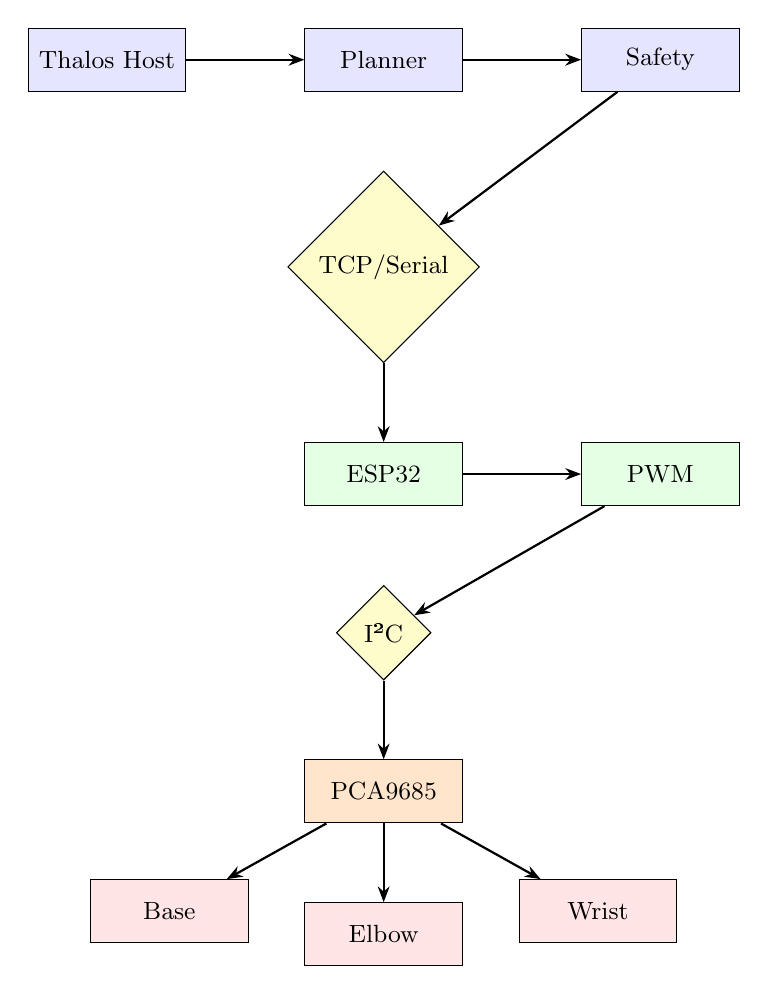
\begin{tikzpicture}[node distance=0.8cm and 1.5cm]

% Host
\node[box, fill=blue!10] (host) {Thalos Host};
\node[box, fill=blue!10, right=of host] (plan) {Planner};
\node[box, fill=blue!10, right=of plan] (saf) {Safety};

% Transport
\node[bus, below=1cm of plan] (tr) {TCP/Serial};

% ESP32
\node[box, fill=green!10, below=1cm of tr] (esp) {ESP32};
\node[box, fill=green!10, right=of esp] (pwm) {PWM};

% I2C
\node[bus, below=1cm of esp] (i2c) {I²C};

% PCA9685
\node[box, fill=orange!20, below=1cm of i2c] (pca) {PCA9685};

% Servos
\node[box, fill=red!10, below left=1cm of pca] (s0) {Base};
\node[box, fill=red!10, below=1cm of pca] (s1) {Elbow};
\node[box, fill=red!10, below right=1cm of pca] (s2) {Wrist};

% Arrows
\draw[arr] (host) -- (plan);
\draw[arr] (plan) -- (saf);
\draw[arr] (saf) -- (tr);
\draw[arr] (tr) -- (esp);
\draw[arr] (esp) -- (pwm);
\draw[arr] (pwm) -- (i2c);
\draw[arr] (i2c) -- (pca);
\draw[arr] (pca) -- (s0);
\draw[arr] (pca) -- (s1);
\draw[arr] (pca) -- (s2);

\end{tikzpicture}
\end{document}
